\documentclass[10pt]{article}

\usepackage{spheric}
%%%TITLE
\title{SPH modeling of fluid-structure interaction (FSI)}
\date{}

%%AFFILIATIONS
\author[$\relax$]{Luhui Han$^\dagger$}
\author[$\relax$]{Xiangyu Hu$^*$}
\affil[$\relax$]{Department of Mechanical Engineering, Technical University of Munich, 85747 Garching, Germany}
\affil[$\relax$]{\email{\dagger}{Luhui.han@tum.de}, \email{*}{Xiangyu.hu}}


%%DOCUMENT
\begin{document}

\maketitle

%\SelectedTopics{}

%%PLEASE PUT YOUR ABSTRACT HERE
\begin{abstract}
This work concerns a numerical modeling of fluid-structure interaction (FSI) in a uniform SPH framework. It combines a transport-velocity SPH scheme \cite{adami2013transport} advancing fluid motions with a total Lagrangian SPH formulation \cite{vignjevic2006sph} dealing with the structure deformations. To remedy the incompleteness of the kernel support at structure boundaries when evaluating strains and inter-particle forces between solid particles, a correction matrix \cite{bonet2002simplified} is employed to restore first order consistency and rotational invariance of Green strain tensor. Since both fluid and solid governing equations are solved in SPH framework, coupling becomes straightforward and meanwhile the momentum of an FSI system is strictly conservative. Several FSI benchmark test cases \cite{bungartz2006fluid} have been performed to validate the modeling and demonstrate its potential.
\begin{figure}[!htb]
\centering
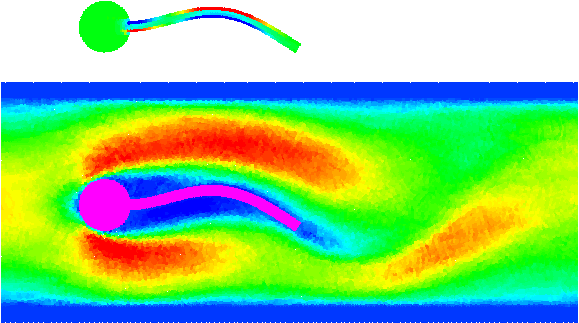
\includegraphics[width=0.8\textwidth]{7-11.pdf}
\caption{Deformation of beam for benchmark case FSI2 \cite{bungartz2006fluid} ($\rho_s/\rho_f = 10$ and $\mathrm{Re} = 100$) with solid
particles colored by contours of von Mises stress (top). Distribution of axial velocity component
$u_x$ (bottom).}\label{fig:7}
\end{figure}

\end{abstract}


%%THE END OF ABSTRACT

\addbib

\end{document}
